
%%%%%%%%%%%%%%%%%%%%%%%%%%%%%%%%%%%%%%%%%%%%%%%%%%%%%%%%%%%%%%%%%%%%%%%%%%%%%%
% This is a template for constructing your project plan document, but
% also to show the use of the l3deliverable class. Use pdflatex and
% bibtex to process the file, creating a PDF file as output (there is
% no need to use dvips when using pdflatex).
%
% Several meta data commands have been implemented to collect
% information such as deliverable identifier, project name etc (see
% below the \date command.

\documentclass{l3deliverable}

%%%%%%%%%%%%%%%%%%%%%%%%%%%%%%%%%%%%%%%%%%%%%%%%%%%%%%%%%%%%%%%%%%%%%%%%%%%%%%
% You can use the svn-multi package to automatically insert version
% control information into your document (an example of how to do this
% is shown below).  Make sure to set the 'svn:keywords' subversion
% property to 'Id' for the source file, for example, type:
%
% svn propset svn:keywords 'Id' d1.tex
%
% in the same directory as your 'd2.tex' file. 
%
% The information between the two $$ will now be updated when you next
% commit the file to your SVN repository.
%
% You can of course, just use this field to insert manual version
% information, e.g. 1.2, 1.2.1 ... instead.


\usepackage{color}
\usepackage{comment}
\usepackage[usenames,dvipsnames,svgnames,table]{xcolor}
\version{3.0}

%%%%%%%%%%%%%%%%%%%%%%%%%%%%%%%%%%%%%%%%%%%%%%%%%%%%%%%%%%%%%%%%%%%%%%%%%%%%%%

\usepackage{url}

%%%%%%%%%%%%%%%%%%%%%%%%%%%%%%%%%%%%%%%%%%%%%%%%%%%%%%%%%%%%%%%%%%%%%%%%%%%%%%
%% Check these macro values for appropriateness for your own document.

\title{System Design Document}

%%authors
\author{
  Dan Tomosoiu \\
  Peeranat Fupongsiripan \\
  Hector Grebbell \\
  Michael Kilian \\
  Anthony Lau \\
}

%%release date 
\date{30 Jan 2013}

\deliverableID{D6}
\project{PSD3 Group Exercise 2}
\team{L}

%%%%%%%%%%%%%%%%%%%%%%%%%%%%%%%%%%%%%%%%%%%%%%%%%%%%%%%%%%%%%%%%%%%%%%%%%%%%%%

\begin{document}

%%%%%%%%%%%%%%%%%%%%%%%%%%%%%%%%%%%%%%%%%%%%%%%%%%%%%%%%%%%%%%%%%%%%%%%%%%%%%%

\maketitle

%%%%%%%%%%%%%%%%%%%%%%%%%%%%%%%%%%%%%%%%%%%%%%%%%%%%%%%%%%%%%%%%%%%%%%%%%%%%%%
%% Standard section for all documents

\section{Introduction}

\subsection{Identification}
This document outlines the proposed design for the Intern Management System. 
\subsection{Related Documentation}
\begin{itemize}
\item{Requirements Specification Document}
\end{itemize}
 

\subsection{Document Status and Schedule}
30/01/2013 - First draft 
%%%%%%%%%%%%%%%%%%%%%%%%%%%%%%%%%%%%%%%%%%%%%%%%%%%%%%%%%%%%%%%%%%%%%%%%%%%%%%
\section{System Overview}
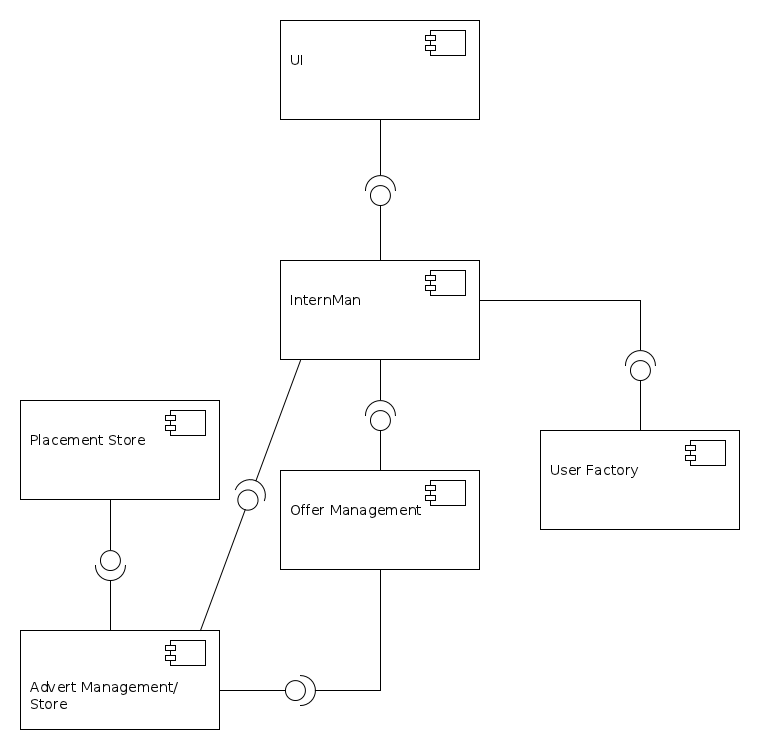
\includegraphics[scale = 0.4]{ComponentDiagram.png}
\\
The proposed system consists of the following components:
\begin{itemize}
\item{InternMan: This component contains an implementation of the InternMan facade provided and can be seen as the 'main' component for the system. }
\item{User Factory: Provides methods for creating new users of different types, storing created users and fetching users from this store. This component also provides
services for authenticating a user's login credentials using a stored username/password combination.}
\item{Offer Management: Handles offers made to students.}
\item{Advert Management/Store: This component provides the necessary services to create and view adverts, associated these with an employer account, etc. It simultaneously
manages the storage and retrieval of adverts from an appropriate source.}
\item{Placement Store: Provides services for manipulating internships and associating these with an approriate role.}
\end{itemize}

%%%%%%%%%%%%%%%%%%%%%%%%%%%%%%%%%%%%%%%%%%%%%
\section{Component Breakdown}

%%%%User factory
\subsection{User Factory}
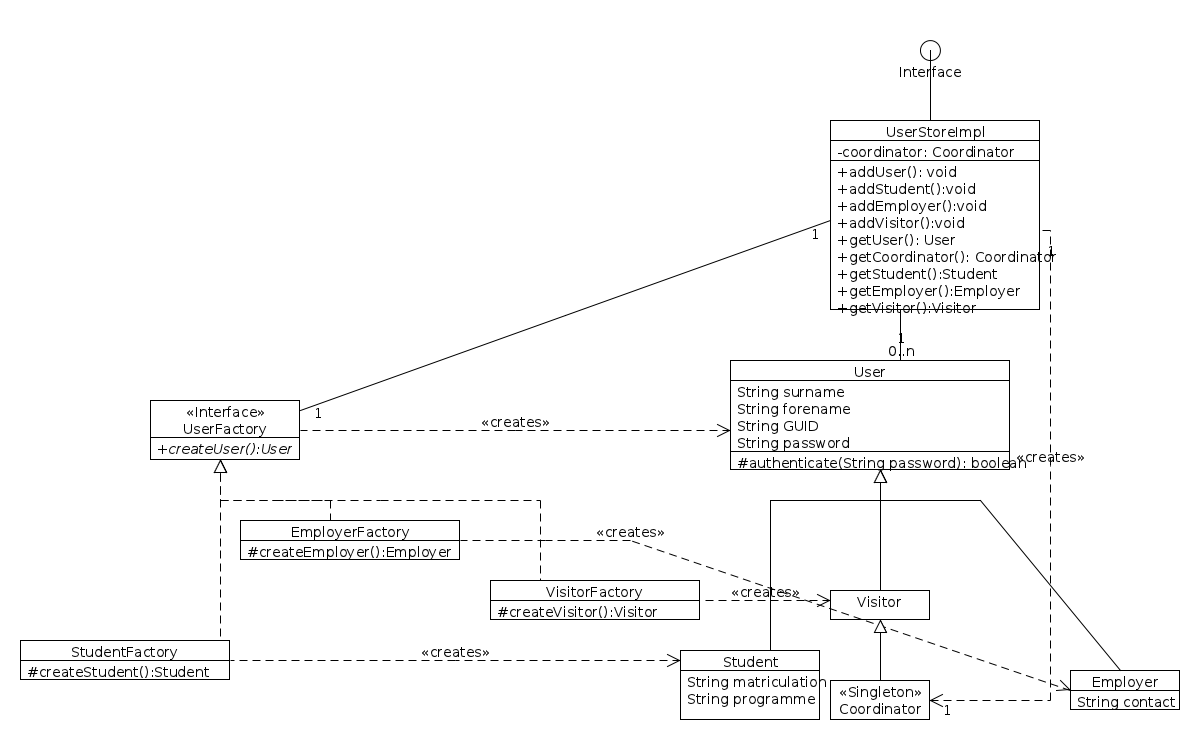
\includegraphics[scale = 0.35]{UserFactoryComponent.png}
\subsubsection{Description and Rationale}
There is a need to create many different categories of user in the system who share attributes and methods. For example all users must be able to log in using a method
to authenticate an input password. In this situation it is appropriate to employ the factory design pattern for the creation of generic users, visitors, students and employers.
The coordinator is not instantiated by a factory, but instead is implemented according to the singleton design pattern. \\
UserStoreImpl groups the methods of these factories and entities together to provide methods for creating and fetching each class of user. For the moment the exact 
means by which these users will be stored has not been decided, but this should also be handled by UserStoreImpl. The method set for UserStoreImpl is equivalent to the API for 
the UserFactory component.
\subsubsection{API}
UserStoreImpl implements UserStore

\textbf{Methods}
\\
%addUser
\textbf{public void addUser(String surname, String forename, String GUID, String password)}\\
Adds a new user to the store.\\
\textbf{Parameter}\\
String surname\\
String forename\\
String GUID\\
String password\\
\\
\\
%addVisitor
\textbf{public void addVisitor(String surname,String forename,String GUID, String password)}\\
Adds a new visitor to the store\\
\textbf{Parameter}\\
String surname\\
String forename\\
String GUID\\
String password\\
\\
\\
%addStudent
\textbf{public void addVisitor(String surname,String forename,String GUID, String password,String matriculation,String programme)}\\
Adds a new student to the store\\
\textbf{Parameter}\\
String surname\\
String forename\\
String GUID\\
String password\\
String matricaulation\\
String programme\\
\\
\\
%addEmployer
\textbf{public void addVisitor(String surname,String forename,String GUID, String password,String contact)}\\
Adds a new employer to the store\\
\textbf{Parameter}\\
String surname\\\
String forename\
String GUID\\
String password\\
String contact\\
\\
\\
%getUser
\textbf{public User getUser(String GUID, String password)}\\
Returns a user specified by the GUID, if authentication is successful.\\
\textbf{Return} the user specified by GUID, if the password is a match\\
\textbf{Parameter}\\
String GUID\\
String password\\
\\
\\
%getVisitor
\textbf{public Visitor getVisitor(String GUID, String password)}\\
Returns a visitor specified by the GUID, if authentication is successful.\\
\textbf{Return} the visitor specified by GUID, if the password is a match\\
\textbf{Parameter}\\
String GUID\\
String password\\
\\
\\
%getStudent
\textbf{public Student getVisitor(String GUID, String password)}\\
Returns a Student specified by the GUID, if authentication is successful.\\
\textbf{Return} the student specified by GUID, if the password is a match\\
\textbf{Parameter}\\
String GUID\\
String password\\
\\
\\
%getEmployer
\textbf{public Visitor getVisitor(String name, String password)}\\
Returns a visitor specified by the name if authentication is successful.\\
\textbf{Return} the user specified by name, if the password is a match\\
\textbf{Parameter}\\
String name\\
String password\\
\\
\\
%%%%%OfferManager
\subsection{Offer Management}
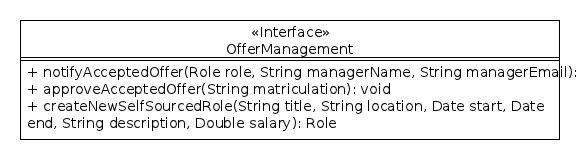
\includegraphics[scale = 0.5]{OfferManagement.png}
\\
\subsubsection{Description and Rationale}
TODO
\subsubsection{API}
TODO

%%%%%Advert Management/Store
\subsection{Advert Management/Store}
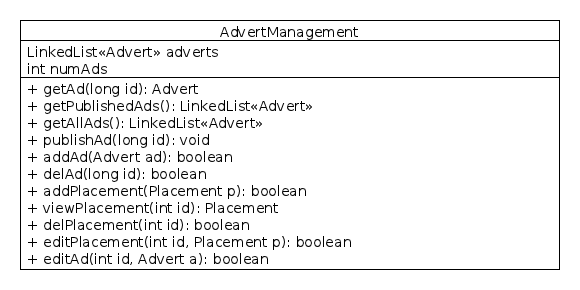
\includegraphics[scale = 0.5]{adStore.png}
\\
\subsubsection{Description and Rationale}
TODO
\subsubsection{API}
TODO

%%%%%Placement Store
\subsection{Placement Store}
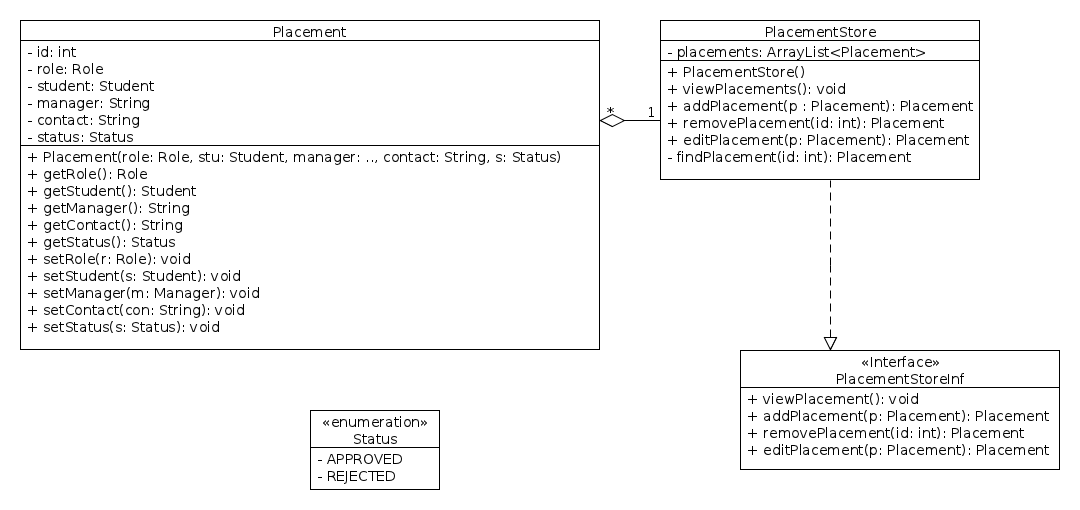
\includegraphics[scale = 0.4]{ClassDiagram_PlacementStore.png}
\\
\subsubsection{Description and Rationale}
TODO
\subsubsection{API}
\textbf{Interface PlacementStoreInf}

\textbf{Methods}\\
%viewPlacements
\textbf{public void viewPlacements()}\\
Prints out all existing placements.
\\
\\
%addPlacement
\textbf{public Placement addPlacement( Placement p )}\\
Add new placement.\\
\textbf{Return: }Placement p added if successful, otherwise null.\\
\textbf{Parameters}\\
Placement p\\
\\
\\
%removePlacement
\textbf{public Placement removePlacement(int id)}\\
\textbf{Return: }Placement with identification number id removed if successful , otherwise null.\\
\textbf{Parameters}\\
int id\\
\\
\\
%editPlacement
\textbf{public Placement editPlacement(Placement p) }\\
Edits existing placement.\\
\textbf{Return: }Placement edited if successful, null otherwise.\\
\textbf{Parameters}\\
Placement p\\
\\
\\
%%%%Class Placement
\textbf{Class Placement}\\
Contains details about the internship including the student taking and role involved.\\
\\
\textbf{public Placement(Role role, Student student, String manager , String contact, Status status)}\\
\textbf{Parameters}\\
Role role\\
Student student\\
String manager\\
String contact\\
Status status\\
\\
\\
\textbf{public Role getRole()}\\
\textbf{Return: }Role of placement if exists, null otherwise.\\
\textbf{Parameters}\\
\\
\\
\textbf{public Student getStudent()}\\
\textbf{Return: }Student secured the placement , null otherwise.\\
\textbf{Parameters}\\
\\
\\
\textbf{public String getManager()}\\
\textbf{Return:}Manager if exists, null otherwise.\\
\textbf{Parameters}\\
\\
\\
\textbf{public String getContact()}\\
\textbf{Return: }Contact details, if exists, null otherwise.\\
\textbf{Parameters}\\
\\
\\
\textbf{public Status getStatus()}\\
\textbf{Return: }returns the status of a particular placement (value can be either APPROVED OR REJECTED)\\
\textbf{Parameters}\\
\\
\\
\textbf{setRole(Role r)}\\
\textbf{Return:}\\
\textbf{Parameters}\\
Role r\\
\\
\\
\textbf{setStudent(Student s)}\\
\textbf{Return:}\\
\textbf{Parameters}\\
Student s\\
\\
\\
\textbf{setManager(String m)}\\
\textbf{Return:}\\
\textbf{Parameters}\\
String m
\\
\\
\textbf{setContact(String c)}
\textbf{Return:}
\textbf{Parameters}
String c\\
\\
\\
\textbf{setStatus(Status s)}\\
\textbf{Return:}\\
\textbf{Parameters}\\
Status s\\
\\
%%%%%%%%%%%%%%%%%%%%%%%%%%%%%%%%%%%%%%%%%%%%%%%%%%%%%%%%%%%%%%%%%%%%%%%%%%%%%%

\appendix

%Including expansions of non-standard abbreviations and acronyms and
%other key definitions.  You may find it useful to maintain a glossary
%as a shared section amongst all your PSD documents. using the
%%API  - Application programming interface\\
PSD  - Professional Software Development\\
PSD3 - Professional Software Development 3\\
UML  - Unified Modeling Language\\

\section{Glossary}
\item{UML - Unified Modelling Language}
\item{API - Application Programming Interface}
\item{PSD/PSD3 - Professional Software Development (3)}


\end{document}
%%%%%%%%%%%%%%%%%%%%%%%%%%%%%%%%%%%%%%%%%%%%%%%%%%%%%%%%%%%%%%%%%%%%%%%%%%%%%%
